\documentclass[a4paper, 12pt]{article}
\usepackage{physics, amsmath, amsfonts, fixmath, geometry, tikz, pgf, multirow, hyperref, amsfonts,amssymb, mathtools, physics, xcolor, siunitx, subcaption,tcolorbox}


\pdfpagewidth 8.5in
\pdfpageheight 11in
\headheight 0pt
\headsep 0pt
\footskip .25in
\marginparwidth 0pt
\marginparsep 0pt
\oddsidemargin \dimexpr 1in -1in
\topmargin \dimexpr 1in -1in
\textwidth \dimexpr \pdfpagewidth -2\oddsidemargin -2in
\textheight \dimexpr \pdfpageheight -2\topmargin -2in
%Commands

\newtcolorbox{boxes}[3][]
{
	colframe = #2!25,
	colback  = #2!10,
	coltitle = #2!40!black,  
	title    = {\textbf{#3}},
	#1,
}
\usepackage{graphicx}
\usepackage{xepersian}
\usepackage{braket}
\settextfont[]{XB Niloofar}
\title{\textbf{
بدست آوردن سیستماتیک گروه هموتوپی اول فضاهای توپولوژیک
\author{حسین محمدی}
}}
\date{}

\begin{document}
\maketitle
شیوه‌ای که در کلاس برای بدست آوردن گروه هموتوپی اول پی گرفتیم، به نظر گنگ بود و حتی جاهایی من به اشکال خوردم. اما روش کامل‌تر و سیستماتیک‌تر کتاب درسی به ما کمک می‌کند که با به کار بستن چند قانون، گروه هموتوپی رو بدست بیاریم.

\noindent
روش کار به این صورته:
\begin{enumerate}
	\item مثلث‌بندی معتبر$K$  از فضای توپولوژیک ارائه کنید.
	\item از مثلث بندی $K$
	یک زیرقسمت
	\LTRfootnote{Subcomplex} 
	$L$  جدا کنید به طوری که:
	\begin{itemize}
		\item $L$ شامل تمامی راس‌های مثلث‌بندی 
		$K$ بشود.
		
		\item چندوجهی 
		$|L|$
		   همبند ساده و مسیری باشد. 
	\end{itemize}
	\item به هر 
	\lr{1-simplex}
	به شکل 
	$(v_i,v_j)$
	از 
	$K-L$
	یک مولد گروه به فرم
	$g_{ij}$
	نسبت بدهید.
	\item اگر یک 
	\lr{2-simplex}
	به فرم 
	$(v_i,v_j,v_k)$
	و
	$(i<j<k)$
	در $K$ هست؛ قید 
	$g_{ij}g_{jk} = g_{ik}$
	را به مولدها اعمال کنید.
	\item به هر 
	\lr{1-simplex}
	 از زیرقسمت $L$، مولد بدیهی رو نسبت بدید.
	\item گروه هموتوپی فضاتون، همان گروهی است که با مولدهای بالا و قیدهای بالا تولید میشه.
\end{enumerate}

به عنوان مثال بیایید فضای 
$\mathbb{R}\text{P}^2$
 رو بررسی کنیم که توی کلاس در بدست آوردن گروهی هموتوپیش ناموفق بودیم.
 
 اول مثلث بندی شکل 
 \ref{rp2tri}
 رو براش در نظر می‌گیریم.
 \begin{figure}[h]
 	\centering{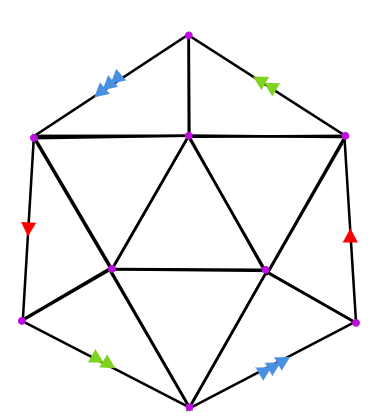
\includegraphics[scale=.7]{Pics/1.png}}
 	\caption{مثلث بندی از 
 	$\mathbb{R}\text{P}^2$
 	}
 	\label{rp2tri}
 \end{figure}
 
  در مرحله دوم، نقاط این مثلث بندی رو نام‌گذاری می‌کنیم؛ توجه کنید که نقاطی که تحت عمل 
  \lr{Identification}
  یکسان می‌شوند، باید با یک شماره نام‌گذاری بشوند. (شکل
  \ref{pic2}
  )
   \begin{figure}[h]
  	\centering{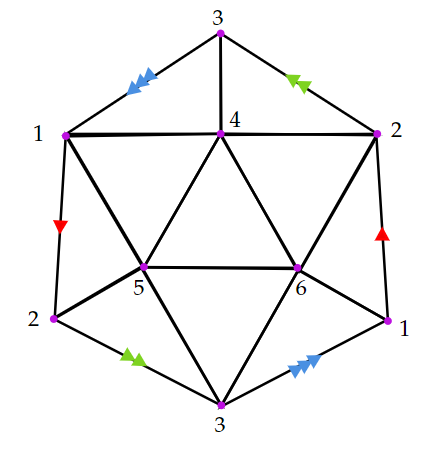
\includegraphics[scale=.7]{Pics/2.png}}
  	\caption{شماره‌گذاری نقاط مثلث‌بندی
  	}
  	\label{pic2}
  \end{figure}
  
  \noindent
  بعد بیایید زیرقسمت 
  $L$
  رو مشخص کنیم، این زیرقسمت باید شامل تمامی نقاط غیریکسان بشه و همچنین باید همبند ساده و مسیری باشه. (شکل 
  \ref{pic3}
  و قسمت خاکستری رنگ.
  )
     \begin{figure}[h]
  	\centering{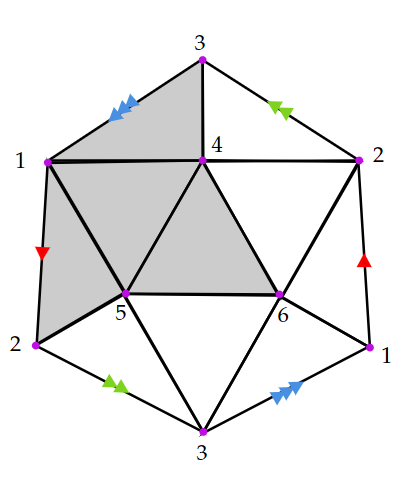
\includegraphics[scale=.7]{Pics/3.png}}
  	\caption{بدست آوردن زیرقسمت
  	$L$
  	  	}
  	\label{pic3}
  \end{figure}
  
  \noindent
  حالا بیایید دونه به دونه قوانین ۴ تا ۶ رو روی این مثلث‌بندی اعمال کنیم. اسم مولد مسیر 
  $23$
  رو می‌گذاریم 
  $x$
  (شکل 
  \ref{pic4}
  )
       \begin{figure}[h]
  	\centering{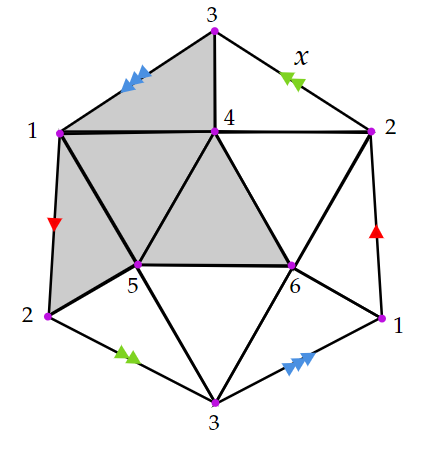
\includegraphics[scale=.7]{Pics/4.png}}
  	\caption{مثلث‌بندی نهایی	
  	}
  	\label{pic4}
  \end{figure}
  و مطابق قانون ۴ برای
  \lr{3-simplex}
  متشکل از 
  $(234)$
  خواهیم داشت:
  \[
  g_{23}g_{34} = g_{24}
  \]
  توجه‌کنید که چون یال 
  $(34)$
  خودش بخشی از 
  $L$
  هست پس مولدش بدیهیه، پس نتیجه میشه که 
  $g_{24} = x.e = x$.
  
  همین کار رو برای وجه‌های 
  $(246) , (126) , (316) , (365) $
  انجام بدیم، مشابها نتیجه میشه که:
  \begin{equation*}
  	g_{26} = g_{16} = g_{36} = g_{35} = x
  \end{equation*}
   اما در مورد وجه 
   $(235)$
   توجه کنید که شرایط یک کم خاص تره.
   \[
   g_{23}g_{35} = g_{25}
   \]
   
  چون
  $(25) \in L$
  پس 
  $g_{25} = e$
   همچنین داشتیم 
   $g_{23} = g_{35} = x$
   ، پس قید آخر نتیجه میده که $x^2=e$.
   
   پس گروه هموتوپی اول فضای 
  $\mathbb{R}\text{P}^2$
  با تک عضو 
  $x$ تولید میشه که مرتبه‌اش دو هست. این دقیقا همون گروه دوری مرتبه ۲ یا 
  $\mathbb{Z}_2$
  هستش.
  \[
  \pi_1(\mathbb{R}\text{P}^2) = \left < x;x^2\right > =   \mathbb{Z}_2
  \]
  
  
 به این روش می‌تونید گروه هموتوپی فضاهای دیگه رو به شکل کاملا استاندارد بدست بیارید؛ مثلا گروه هموتوپی کره دو و سه بعدی که توی کلاس  به مشکل خورد، به این روش قابل حل کردنه. 
 مثلث‌بندیهایی که توی کلاس حل تمرین دیدیم در حقیقت به معنای درست مثلث بندی نبودند، ولی کار رو فوق العاده ساده‌تر می‌کردند.
 
 در آخر هم دعوتتون می‌کنم تا شکل ۴.۱۶ کتاب رو ببینید و متوجه بشید که چرا گروه هموتوپی فضای 
 $\mathbb{R}\text{P}^2$
 تنها دو عضو داره.
  
  
  







\end{document}